% THIS DOCUMENT IS FOLLOWS THE VOLERE TEMPLATE BY Suzanne Robertson
% and James Robertson
% ONLY THE SECTION HEADINGS ARE PROVIDED
%
% Initial draft from https://github.com/Dieblich/volere
%
% Risks are removed because they are covered by the Hazard Analysis
\documentclass[12pt]{article}
\usepackage{graphicx}
\usepackage{booktabs}
\usepackage{tabularx}
\usepackage{hyperref}
\usepackage{enumerate}
\usepackage{amsmath}
\hypersetup{
  bookmarks=true,         % show bookmarks bar?
  colorlinks=true,      % false: boxed links; true: colored links
  linkcolor=red,          % color of internal links (change box color
  % with linkbordercolor)
  citecolor=green,        % color of links to bibliography
  filecolor=magenta,      % color of file links
  urlcolor=cyan           % color of external links
}

\newcommand{\lips}{\textit{Insert your content here.}}

%% Comments

\usepackage{color}

\newif\ifcomments\commentstrue %displays comments
%\newif\ifcomments\commentsfalse %so that comments do not display

\ifcomments
\newcommand{\authornote}[3]{\textcolor{#1}{[#3 ---#2]}}
\newcommand{\todo}[1]{\textcolor{red}{[TODO: #1]}}
\else
\newcommand{\authornote}[3]{}
\newcommand{\todo}[1]{}
\fi

\newcommand{\wss}[1]{\authornote{blue}{SS}{#1}} 
\newcommand{\plt}[1]{\authornote{magenta}{TPLT}{#1}} %For explanation of the template
\newcommand{\an}[1]{\authornote{cyan}{Author}{#1}}

%% Common Parts

\newcommand{\progname}{ProgName} % PUT YOUR PROGRAM NAME HERE
\newcommand{\authname}{Team \#, Team Name
\\ Student 1 name
\\ Student 2 name
\\ Student 3 name
\\ Student 4 name} % AUTHOR NAMES                  

\usepackage{hyperref}
    \hypersetup{colorlinks=true, linkcolor=blue, citecolor=blue, filecolor=blue,
                urlcolor=blue, unicode=false}
    \urlstyle{same}
                                


\begin{document}

\title{Software Requirements Specification for \progname: Document
Management System}
\author{\authname}
\date{\today}

\maketitle

~\newpage

\pagenumbering{roman}

\tableofcontents

~\newpage

\section*{Revision History}

\begin{tabularx}{\textwidth}{p{3cm}p{2cm}X}
  \toprule {\textbf{Date}} & {\textbf{Version}} & {\textbf{Notes}}\\
  \midrule
  Date 1 & 1.0 & Notes\\
  Date 2 & 1.1 & Notes\\
  \bottomrule
\end{tabularx}

~\\

~\newpage
\section{Purpose of the Project}
\subsection{User Business}
The City of Hamilton's Water Division is responsible for the
treatment and distribution of drinking water and the collection and
treatment of wastewater throughout the City of Hamilton. Many pumping
stations are located throughout the City to perform this work. The
maintenance and upkeep of these facilities is crucial to ensure
unimpeded service. The facilties team at Hamilton Water requires an
application to assist in the management and security of these
stations, as there is not a robust system currently in place. For
detailed information on the problems the application should address,
refer to the problem statement
\href{https://github.com/Spitgranger/capstone/blob/main/docs/ProblemStatementAndGoals/ProblemStatement.pdf}{here}.
\subsection{Goals of the Project}
The development of this application will greatly improve the
efficiency and transparency of facility management at Hamilton Water
and improve station security. For detailed information on the goals
of this project, refer to Section 2: Goals
\href{https://github.com/Spitgranger/capstone/blob/main/docs/ProblemStatementAndGoals/ProblemStatement.pdf}{here}.
\section{Stakeholders}
\subsection{Client}

\begin{itemize}
  \item Matt Yakymyshyn (P.Eng)
    \begin{itemize}
      \item[-] Role: Senior Project Manager of Technical Services
      \item[-] Interest: Team leader for the facilities team within
        Technical Services who are the primary group responsible for
        maintaining facility infrastructure at pumping stations.
        Primary contact at the City for the capstone team.
    \end{itemize}
\end{itemize}

\subsection{Customer}

\begin{itemize}
  \item Technical Services team
    \begin{itemize}
      \item[-] Role: Primary user within Hamilton Water
      \item[-] Interest: As the primary stakeholder, the requirements
        of this project are aimed at their specific needs. Their main concern
        is that station documentation is managed as a single source of truth,
        and is easily distributed/retrieved with relevant parties.
    \end{itemize}
\end{itemize}
\subsection{Other Stakeholders}

\begin{itemize}
  \item Supervisory Control and Data Acquisition (SCADA) team
    \begin{itemize}
      \item[-] Role: Responsible for the control system controlling
        the treatment process.
      \item[-] Interest: The SCADA team also manages contractors and is
        interested in accessing and updating documentation maintained
        in this system.
      \item[-] They will have valuable input regarding existing City
        platforms and technologies, as well as how technology can be
        integrated into pumping stations.
    \end{itemize}
  \item Corporate Security

    \begin{itemize}
      \item[-] Role: Pumping Station Security
      \item[-] Interest: Provide feedback on any system involving station
        access.
    \end{itemize}
\end{itemize}

\subsection{Hands-On Users of the Project}
\begin{itemize}
  \item Facilities project managers
    \begin{itemize}
      \item[-] The facilities project managers will be using the application
        daily to perform a variety of tasks. This includes verifying work was
        performed by contractors, accessing station documentation to share with
        contractors and internal staff, receiving signed forms and storing in a
        manner which is associated to the signee, and other tasks.
        They will have to be able to achieve all their needed requirements
        through the applications user interface, and will be a critical
        stakeholder to receive feedback from through user testing.
    \end{itemize}
  \item Facilities co-op students
    \begin{itemize}
      \item[-] Facilities co-op students will be using the application to
        physically authenticate on site when performing inspections,
        scoping work, and verifying completion of work.
    \end{itemize}
  \item Facilities contractors
    \begin{itemize}
      \item[-] Many contractors access pumping stations daily. They will
        interact with the application each time they perform facilities related
        work at the station. Interactions would include uploading and
        receiving documentation, and authenticating their presence on site
        to verify completion of work.
        Contractors come from a wide range of backgrounds depending on their
        trade, but are typically skilled workers in a particular field and are
        of working age (18 - 65 years old).
    \end{itemize}
  \item Facilities sub-contractors
    \begin{itemize}
      \item[-] Many contractors employ sub-contractors as part of their work.
        While these subcontractors work for the contractor who hired them, they
        will still require access to the application to authenticate on site
        and access site information. Their roles and interactions
        will be similar to contractors, except they will be much less familiar
        with the application and may only use it for a short duration as they
        are not regular workers.
    \end{itemize}
\end{itemize}
\subsection{Personas}

\begin{itemize}
  \item Greg: A facilities manager
    \begin{itemize}
      \item[-] Greg has a few tasks to complete this morning at work.
        He sees that another department has requested compliance documentation
        on crane inspections for the ministry, so he signs onto SyncMaster to
        retrieve the current version of these documents for each of these sites.
        While on the application, he receives a notification that a contractor
        he manages authenticated at site to complete a work order, but the
        application identified they had not completed their health and safety
        training. Greg prompts the system to issue this training to them, and
        runs a report on this contractor to see if any other employees of
        theirs require their training soon.
    \end{itemize}
  \item Nancy: A newly onboarded contractor
    \begin{itemize}
      \item[-] Nancy is a plumber who is servicing her first work order after
        being hired by ``Worldly Plumbing''.
        Her company has notified her of the application she must use to
        authenticate for the work. When she authenticates, she is notified that
        the device she is servicing is located within a confined space
        and that she must sign and return a hazard assessment form and proof
        of confined space training.
    \end{itemize}
\end{itemize}
\subsection{Priorities Assigned to Users}

\begin{itemize}
  \item Key users
    \begin{itemize}
      \item[-] Facilities managers. They are the primary stakeholder of the
        application and it is intended to be a tool to greatly improve the
        efficiency of their work.
    \end{itemize}
  \item Secondary users
    \begin{itemize}
      \item[-] Contractors. They will frequently use the system, but their
        needs are secondary to the key users.
    \end{itemize}
\end{itemize}
\subsection{User Participation}

\begin{itemize}
  \item Facilities managers will be frequently consulted throughout the
    duration of this project to demonstrate prototypes, receive feedback,
    and conduct user testing.
  \item Co-op students can also be consulted for user testing. They
    tend to have more availability for longer durations and will be
    able to provide insight into how a less experienced user
    interacts with the system.

\end{itemize}
\subsection{Maintenance Users and Service Technicians}
The facilities managers will be responsible for ensuring that day-to-day data
is added to the application appropriately. The team does not have a dedicated
software position, so maintainability of the technical aspects of the
application would need to be brought to the IT division of the City
when the project reaches that stage.

\section{Mandated Constraints}
\subsection{Solution Constraints}
\begin{enumerate} [{C-SOL}1.]
  \item System must be cloud-based to fit in with current existing systems at
    the City of Hamilton.
\end{enumerate}

\subsection{Implementation Environment of the Current System}
To understand the current practices at the City of Hamilton see the
\textit{Problem} section of the Problem Statement and Goals
\href{https://github.com/Spitgranger/capstone/blob/main/docs/ProblemStatementAndGoals/ProblemStatement.md#11-problem}
{here}.

\subsection{Partner or Collaborative Applications}
N/A
\subsection{Off-the-Shelf Software}
\begin{enumerate} [{C-OTS}1.]
  \item The system must integrate with Sharepoint to synchronize documents in
    Sharepoint with documents in the system.
  \item The system must integrate with Infor EAM, to show the status of work
    orders associated with a document.
  \item The system must integrate with MySDS to show relevent relevant SDS
    documents to users on a given site.
\end{enumerate}

\subsection{Anticipated Workplace Environment}
\begin{enumerate} [{C-AWE}1.]
  \item The workplace is an industrial environment. The application must
    be usable in a manner which ensures worker health and safety per the
    City's health and safety procedures.
  \item The workplace is a hybrid environment of in-office and on-site
    work. The application should be accessible from both environments, as
    the requirements permit.
  \item Many stations are accessed from outdoors and the user is exposed to
    the current weather conditions. The application must be usable in any
    weather condition.
\end{enumerate}

\subsection{Schedule Constraints}
\begin{enumerate} [{C-SCH}1.]
  \item A requirement is to integrate with the Infor EAM system the city intends
    on using however, this system will not be available until
    February 2025, so no testing can be done on this system until then.

  \item The project deadline is April 2, 2025.
\end{enumerate}

\subsection{Budget Constraints}
\begin{enumerate} [{C-BDG}1.]
  \item Total expenses up until April 2, 2025 must not exceed \$750.
\end{enumerate}

\subsection{Enterprise Constraints}
N/A

\section{Naming Conventions and Terminology}
\subsection{Glossary of All Terms, Including Acronyms, Used by Stakeholders
involved in the Project}
\begin{itemize}
  \item BAS: Building Automation System.
  \item BCOS: Beyond Compliance Operating System.
  \item CMMS: Computerized Maintenance Management System.
  \item Confined Space: A partially or fully enclosed space, not designed for
    continuous human occupancy, which has the potential for atmospheric hazards.
  \item Controlled Space: A City defined space which has the potential to
    become a confined space.
  \item CSE: Confined Space Entry
  \item Dry Well: A room which houses industrial equipment such as pumps
    and valves.
  \item Hazard Assessment Form: A form outlining potential
    hazards at a location.
  \item Hot Works: Work which produces ignition sources.
    Requires an accompanying hot works permit.
  \item HVAC: Heating, Ventilation, and Air Conditiong.
  \item Infor EAM: An Enterprise Asset Management system.
  \item PMATS: Plant Maintenance and Technical Services.
  \item PO: Purchase Order.
  \item PPE: Personal Protective Equipment.
  \item SCADA: Supervisory Control and Data Acquisition.
  \item SDS: Safety Data Sheets.
  \item Wet Well: A portion of a wastewater pumping station which receives
    and temporarily stores wastewater.
\end{itemize}

\section{Relevant Facts And Assumptions}
\subsection{Relevant Facts}
\begin{itemize}
  \item There are over 100 pumping stations throughout the City.
  \item There are dozens of service contracts, and many contractors
    and staff accessing stations each day.
  \item Some stations are in remote locations and may have poor cell signal.
  \item Some properties have multiple stations at the same site.
  \item Certain stations have special entry procedures.
\end{itemize}

\subsection{Business Rules}
\begin{itemize}
  \item External contractors do not have access to the internal network.
  \item Only authorized users can approve new procedures.
  \item There is work at stations performed through a work order
    and routine work which doesn't have a work order.
  \item Employee collective agreements have restrictions on the release of
    GPS logs and video recording, which would require their approval.
\end{itemize}
\subsection{Assumptions}
\begin{itemize}
  \item Our project will focus on the application itself
    and our team will implement an authentication system adequate for our
    development. When the City integrates our application into their systems
    they would replace our authentication system with one that meets their
    detailed cybersecurity specifications.
  \item The existing entry and exit procedure for stations is not modified
    and our application will coexist with it.
\end{itemize}
\section{The Scope of the Work}
\subsection{The Current Situation}
The process currently employed by the stakeholder is predominantly a manual one.
Currently, contractor management is a time-consuming and manual effort. The
following list identifies the current situation faced by the City:
\begin{itemize}
  \item To distribute new or revised documentation to contractors,
    the City sends the documents manually through email. There are no
    automated processes in place and this work flow is done manually
    for each document. There are dozens of contractors which these
    documents need to be distributed to, and those contractors
    themselves also change over time. The list of these contractors
    is also managed manually.
  \item Verification of work performed by contractors currently
    requires a physical visit to site. There is no automated process
    to collect information such as photos of the work performed,
    other than manually through email.
  \item It is currently difficult to know whether the labour cost
    billed by the contractors on their invoices is reflective of the
    actual work performed, as that information is only recorded in a
    physical logbook at each site and is not electronic. A contractor
    could overcharge for the work and it would be difficult to prove
    that their bill is inaccurate.

\end{itemize}

\subsection{The Context of the Work}
The below figure illustrates a high-level context model of the adjacent systems:
\begin{figure}[h]
  \centering
  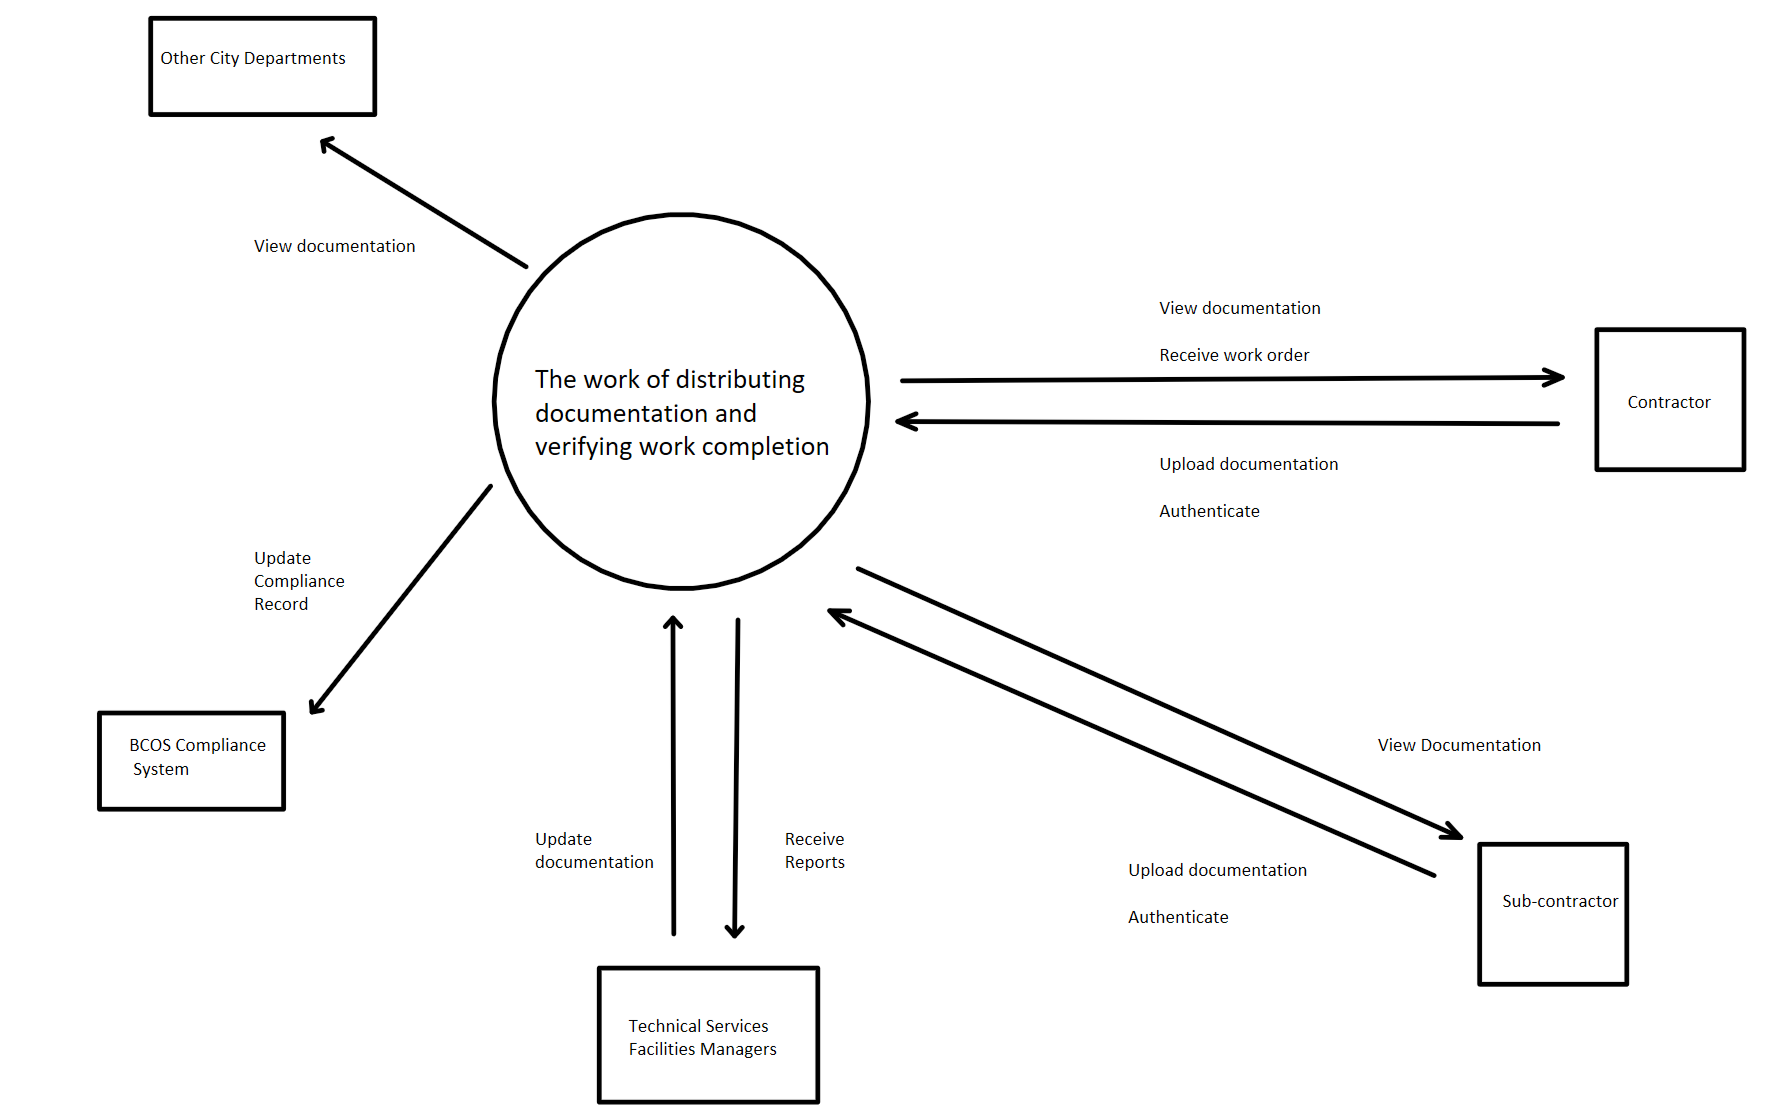
\includegraphics[width=1\textwidth]{4G06A-context-model.png}
  \caption{Context model}
\end{figure}

\subsection{Work Partitioning}
\begin{tabular}{|l|l|}
  \hline
  \textbf{Event Name} & \textbf{Input and Output} \\
  \hline
  1. Contractor Login & Contractor email and one time password (in) \\
  \hline
  2. Contractor Location Verification & GPS location (in) \\
  \hline
  3. Staff Login & Staff email and password (in) \\
  \hline
  4. Sign Document & unsigned document (in), signed document (out) \\
  \hline
  5. Upload Report & report file (in) \\
  \hline
  6. Export Reports & report specifications (in), report data (out)\\
  \hline
  7. View Station Entry Protocols & Station location (in), entry
  protocol (out)\\
  \hline
  8. Add Contractor to System & Contractor information (in) \\
  \hline
  9. View Contractor Summary & Contractor name (in), contractor data (out) \\
  \hline
  10. Certification Expiry & notice of document expiration to staff (out) \\
  \hline
\end{tabular}

\subsection{Specifying a Business Use Case (BUC)}
The below points identify the business use cases for each of the
business events by number in section 6.3.\\

\begin{enumerate}
  \item Contractor authenticates themselves to City systems, proving that they
    are authorized to be provided City information.\\
  \item Contractor proves they are at a site for transparency when work is being
    completed.\\
  \item Staff authenticates themselves as authorized to view private data.\\
  \item Sign a document for contractual or regulatory purposes.\\
  \item Documents are stored for record keeping and relevant stakeholders
    are notified as necessary.\\
  \item Export data of a specific type specified by the user. For example, all
    crane inspections in the last year.\\
  \item View a procedure of how staff and contractors must access a specified
    station.\\
  \item New contractors are frequently onboarded, and their information is
    recorded by the facilities managers.\\
  \item Facilities managers commonly need to see which employees of a contractor
    are due for their health and safety training, WSIB expiry, etc.\\
  \item When a piece of documentation has expired, the next version needs to be
    put in place by staff to replace the expired version.\\
\end{enumerate}

\section{Business Data Model and Data Dictionary}
\subsection{Business Data Model}
\lips
\subsection{Data Dictionary}
\lips

\section{The Scope of the Product}
\subsection{Product Boundary}

The table below displays aspects of the application which are in scope and
aspects which are out of scope. \\

\begin{tabular}{|p{0.45\linewidth}|p{0.45\linewidth}|}
  \hline
  \textbf{In Scope} & \textbf{Out of Scope} \\
  \hline
  Designing the application in a way where it is able to interact with the
  external work order system is a stretch goal.& Designing any aspects of a full
  work order system is out of scope for this project. \\
  \hline
  The application will implement an authentication system sufficient to
  demonstrate contractors authenticating themselves onto sites. & A thorough
  cybersecurity analysis for the authentication is not in scope as it is not the
  primary focus for the applications functionality. \\
  \hline
\end{tabular}

\subsection{Product Use Case Table}

\begin{tabular}{|p{0.45\linewidth}|p{0.45\linewidth}|}
  \hline
  \textbf{User}& \textbf{Use Case} \\
  \hline
  Facilities Manager & - View contractor authentication data to determine that
  a contractor was at a particular location and completed the work expected
  and invoiced accordingly. \\
  & - Generate a report of compliance documentation in the system for easy
  sharing to relevant third parties. \\
  & - Manage the health and safety documentation and training status of
  their contracts.\\
  \hline
  Contractors & - Authenticate their arrival to site to confirm work is being
  performed.\\
  & - Access station entry and exit procedures, hazard forms, and other safety
  information which should be known when accessing the station.\\
  & - Sign and acknowledge forms and return them to the City.\\
  & - Upload photographs, documents, and comments about work done at
  the station. \\
  \hline
\end{tabular}

\subsection{Individual Product Use Cases (PUC's)}
N/A.
\section{Functional Requirements}
\subsection{Formal Definitions}
\begin{itemize}
  \item Let \(U = \{u_1, u_2, \cdots, u_i\}\) be the set of users in the system.
  \item Let \(R = \{r_1, r_2, \cdots, r_r\}\) be the set of roles (e.g. manager,
    contractor, subcontractor).
  \item Let \(A = \{a_1, a_2, \cdots, a_s\}\) be the set of actions (e.g.
    upload, authenticate, sign, view).
  \item Let \(C = \{c_1, c_2, \cdots, c_t\}\) be the set of compliance
    requirements (e.g. safety training, hazard assesments).
  \item Let \(I = \{l_1, l_2, \cdots, l_q\}\) be the set of allowed locations.
  \item Let \(loc(u_i)\) represent the current location of user \(u_i\).
  \item Let \(D = \{d_1, d_2, \cdots, d_n\}\) be the set of documents.
  \item Let \(hasRole(u_i, r_k)\) represent that user \(u_i \in U\) has a role
    \(r_k \in R\).
  \item Let \(notify(u_m, u_i)\) represent a notification from user
    \(u_m \in U\) to user \(u_i \in U\).
  \item Let \(notify(u_i)\) represent a notification from the system to user
    \(u_i \in U\)
  \item Let \(manages(u_m, u_i)\) represent that user \(u_m \in U\)
    manages user \(u_i \in U\).
  \item Let \(permitted(r_k, a_s, d_j)\) represent that a user with
    role \(r_k \in R\) is permitted to perform action \(a_s \in A\)
    on document \(d_j \in D\)
  \item Let \(requires(a_s, c_t)\) represent that action \(a_s \in A\) requires
    compliance requirement \(c_t \in C\)
  \item Let \(T(u_i) \subset C\) represent the set of completed training for a
    user \(u_i \in U\).
  \item Let \(assoc(d_j, u_i)\) denote that document \(d_j\) is associated with
    user \(u_i\).
  \item Let \(upload(u_i, d_j)\) represent the action of user \(u_i \in U\)
    uploading document \(d_j \in D\).
  \item Let \(performAction(u_i, a_s, d_j)\) represent that user \(u_i \in U\)
    performs action \(a_s \in A\) on document \(d_j \in D\).
  \item Let \(expired(c_i)\) represent that compliance document \(c_i \in C\)
    has expired.
\end{itemize}
\subsection{Formal Expressions}
\begin{enumerate}
  \item \(\forall u_i \in U, \forall d_j \in D, \forall r_k \in R, \forall a_s
    \in A: \)
    \begin{align*}
      hasRole(u_i, r_k) \land permitted(r_k, a_s, d_j) \implies
      performAction(u_i, a_s, d_j)
    \end{align*}
  \item \(\forall u_i \in U, \forall c_t \in C:\)
    \begin{align*}
      (requires(a_s, c_t) \land a_s = sign \implies (c_t \in T(u_i)) \implies
      performAction(u_i, a_s, d_j))
    \end{align*}
  \item \(\forall u_i \in U, \forall d_j \in D:\)
    \begin{align*}
      (loc(u_i) \in L) \implies upload(u_i, d_j)
    \end{align*}
  \item \(\forall u_i \in U, \forall d_j \in D:\)
    \begin{align*}
      (loc(u_i) \notin L) \implies \lnot upload(u_i, d_j)
    \end{align*}
  \item \(\forall u_i \in U, \forall d_j \in D:\)
    \begin{align*}
      sign(u_i, d_j) \implies assoc(d_j, u_i)
    \end{align*}
  \item \(\forall u_i \in U, \forall c_t \in C, \forall u_m \in U:\)
    \begin{align*}
      (manages(u_m, u_i) \land c_t \notin T(u_i)) \implies notify(u_m, u_i)
    \end{align*}
  \item \(\forall u_i \in U, \forall c_t \in C\)
    \begin{align*}
      (expired(c_t) \implies notify(u_i))
    \end{align*}
\end{enumerate}
\subsection{Functional Requirements}
\begin{enumerate} [{FR}1.]
  \item System should support at a minimum the docx, xlsx, and pdf
    file formats for upload and viewing.
  \item Documents in this system must be synchronized with
    Sharepoint, this means any changes in this system must be
    reflected in the corresponding Sharepoint document, and any
    changes to the document in Sharepoint must be reflected in this system.
  \item The system should have different access levels depending on
    the type of user. Only Admin users should be able to change
    access permissions of other users and have read and write
    accesses to all documents in the system. Contractors/general
    users should only have read access to documents and be able to
    sign documents. See (1) in \textbf{Section 9.2 Formal Expressions}.
  \item The current site, work order number, job details, and entry/exit time of
    contractors should be visible to admin users in the system.
  \item The system must implement a form of geolocation verification before
    contractors are able to authenticate and upload documents. See (3) and
    (4) in \textbf{Section 9.2 Formal Expressions}.
  \item The system must notify users when a complicance document has expired.
    See (7) in \textbf{Section 9.2 Formal Expressions}.
  \item The system must store the date, time, name of person, and name of
    document when a user acknowledges a document. See (5) in
    \textbf{Section 9.2 Formal Expressions}.
  \item The system must notify the manager of a contractor when a contractor
    attempts to authenticate and upload documents at a particular site prior to
    completion of required training. See (6) in
    \textbf{Section 9.2 Formal Expressions}.
  \item The system must prevent a user from authenticating or uploading
    documents if the required training for the specific site is not complete.
    See (2) in \textbf{Section 9.2 Formal Expressions}.

\end{enumerate}

\section{Look and Feel Requirements}
\subsection{Appearance Requirements}
\begin{enumerate}[{LF-AP}1.]
  \item The colour palette of the application should align with other
    applications used by the city of Hamilton. \\
    \textbf{Rationale}: Aligning with the look of current
    applications at the city of Hamilton creates a consistent feel
    for current employees using the application.
\end{enumerate}
\subsection{Style Requirements}
\begin{enumerate}[{LF-ST}1.]
  \item The application should have a responsive design which
    considers different screen sizes and orientations. \\
    \textbf{Rationale}: The application may be used on a variety of
    different devices and therefore must be able to account for
    varying screen sizes and orientations.
\end{enumerate}

\section{Usability and Humanity Requirements}
\subsection{Ease of Use Requirements}
\begin{enumerate}[{UH-EU}1.]
  \item Users between the ages of {MIN\_AGE} and {MAX\_AGE},
    regardless of technical expertise, must be able to discover at least 70\% of
    the web application functionality within 10 minutes of being introduced to
    the system without any explaination or training.\\
    \textbf{Rationale}: Usability is of high importance to the users
    of the system. They will be mainly non-technical and must be able
    to learn and use the system quickly if it is to be of any value to them.
  \item The system should provide undo options or warnings for
    irreversible actions and 95\% of users should successfully use
    these features when prompted.\\
    \textbf{Rationale}: It is important to provide users of the systems with
    confirmations or warnings to prevent errors and if they do happen, make it
    easy to recover from them.
\end{enumerate}
\subsection{Personalization and Internationalization Requirements}
N/A
\subsection{Learning Requirements}
\begin{enumerate}[{UH-LR}1.]
  \item Users between the ages of {MIN\_AGE} and {MAX\_AGE} should not take
    more than 10 minutes to a learn feature of the web application after it is
    discovered.\\
    \textbf{Rationale}: A well designed system should give the user
    the most amount of functionality while being easy to understand.
    Users will be able to productive with the system in a short
    amount of time, reducing frustration.
  \item Users between the ages of {MIN\_AGE} and {MAX\_AGE} should be able to
    complete the system onboarding tutorial or walkthrough within 5 minutes,
    and 80\% of users should report feeling confident in using the
    system afterward.\\
    \textbf{Rationale}: It is important that users are able to understand
    system documentation quickly to reduce mental overhead and increase
    productivity.
\end{enumerate}
\subsection{Understandability and Politeness Requirements}
\begin{enumerate}[{UH-UP}1.]
  \item The application must not contain symbols or allusions that
    may be offensive or politically charged.\\
    \textbf{Rationale}: As the system is to be used by people of
    diverse backgrounds and in a professional setting, it is
    important to keep a professional and neutural tone.
  \item System error messages should clearly explain the issue and
    suggest a resolution within 2 sentences. 90\% of users between
    the ages of {MIN\_AGE} and {MAX\_AGE} should report understanding
    the error and being able to resolve the issue without external support.\\
    \textbf{Rationale}: Useful system feedback is crucial since users need to
    know what the system is doing and how it interprets their input in order to
    determine next steps.
\end{enumerate}
\subsection{Accessibility Requirements}
TBD may be in constraints.
\section{Performance Requirements}
\subsection{Speed and Latency Requirements}
\lips
\subsection{Safety-Critical Requirements}
\lips
\subsection{Precision or Accuracy Requirements}
\lips
\subsection{Robustness or Fault-Tolerance Requirements}
\lips
\subsection{Capacity Requirements}
\lips
\subsection{Scalability or Extensibility Requirements}
\lips
\subsection{Longevity Requirements}
\lips

\section{Operational and Environmental Requirements}
\subsection{Expected Physical Environment}
\begin{enumerate} [{OE-PE}1.]
  \item Application should be functional in City of Hamilton, Water
    Division sites and offices.
\end{enumerate}
\subsection{Wider Environment Requirements}
\begin{enumerate} [{OE-WE}1.]
  \item Application should be functional on Mobile and Desktop web
    browser layouts.
  \item Application should be able to run on Chrome, Microsoft Edge,
    and Mobile Browsers.
\end{enumerate}
\subsection{Requirements for Interfacing with Adjacent Systems}
\begin{enumerate} [{OE-IAS}1.]
  \item Application should integrate with existing SharePoint repositories.
  \item Application should be able to provide up-to-date Safety Data
    Sheets from MySDS.
  \item Application should be open for integration with upcoming Work
    Order tracking system in the city's Enterprise Asset Management software.
\end{enumerate}
\subsection{Productization Requirements}
N/A
\subsection{Release Requirements}
\begin{enumerate} [{OE-REL}1.]
  \item A changelog should be generated with every release
    documenting changes in features, requirements and fixes made.
  \item A release is defined as a Revision. Every revision should be
    a major deployment of new features and/or fixes into production.
  \item Expected release of Revision 0: February 1st, 2024
  \item Expected release of Revision 1: March 30th, 2025
\end{enumerate}

\section{Maintainability and Support Requirements}
\subsection{Maintenance Requirements}
\begin{enumerate} [{MS-MTN}1.]
  \item A deployment of the system should take no more than 30 minutes (not
    including testing, and building time).
  \item The build time of the system should be no longer than 10 minutes (not
    including testing time).
  \item All automated tests should be able to run in under 10 minutes
  \item The system should have rigourous unit testing, line coverage should be
    $\ge$ 95\%, branch coverage should be $\ge$ 90\%.
  \item All core functionalities of the system (i.e. Functional Requirements),
    should have both automated end-to-end and unit testing corresponding to them
  \item The project must be able to be maintained by its users, as original
    developers will not be maintaining it after April 2, 2025.
\end{enumerate}
\subsection{Supportability Requirements}
\begin{enumerate} [{MS-SUP}1.]
  \item The application should have user-facing documentation on how to use the
    core functionalities of the system (i.e. functionalities described in
    functional requirements).
  \item The application should have documentation for all API's for future
    maintainers.
  \item The application should have documentation of internal functions and
    abstractions for future maintainers.
  \item The application should have documentation on deployment, so users can
    deploy this application for themselves.
\end{enumerate}
\subsection{Adaptability Requirements}
\begin{enumerate} [{MS-ADP}1.]
  \item The application must be able to run on at least Google Chrome and
    Microsoft Edge browsers.
  \item The application must be able to run on tablets, smartphones, and
    laptops.
  \item The application must be able to run on Android, IOS, and Windows 10
\end{enumerate}

\section{Security Requirements}
\subsection{Access Requirements}
\begin{enumerate} [{SR-AR}1.]
  \item Only authorized contractors and employees should be able to access the
   portal for completing work on site.
  \item Only users with managerial level access should be able to get data on
   contractors and employees.
  \item Only users with administrative access should be able to make changes to
   site settings.
  \item The upload and changing of certain file classes will be tied to
   different access levels.
\end{enumerate}
\subsection{Integrity Requirements}
\begin{enumerate} [{SR-IR}1.]
  \item The application should not allow the addition, removal or modification
   of files by users without proper access and authentication.
  \item The documents displayed should match the appropriate version available
   on SharePoint and/or MySDS.
  \item The application should minimize the amount of bad or incomplete data
   inputted through the portal.
\end{enumerate}
\subsection{Privacy Requirements}
\begin{enumerate} [{SR-PR}1.]
  \item Data transmission will be encrypted.
  \item The application should protect private information in accordance with
   any and all government privacy laws and policies.
\end{enumerate}
\subsection{Audit Requirements}
\begin{enumerate} [{SR-AR}1.]
  \item The application will adhere to any and all audit rules followed by City
   departments.
\end{enumerate}
\subsection{Immunity Requirements}
\begin{enumerate} [{SR-IMR}1.]
  \item The application will be made as secure as feasibly possible within the
   scope of this project to prevent cybersecurity attacks or hacking by
    malicious parties.
\end{enumerate}

\section{Cultural Requirements}
\subsection{Cultural Requirements}
\lips

\section{Compliance Requirements}
\subsection{Legal Requirements}
\begin{itemize}
  \item[CR-L1] The application is to strictly abide by all regulations governing
    the treatment of water and wastewater. This includes, but is not limited
    to the \textit{Safe Drinking Water Act} (SDWA), 2002, the
    \textit{Ontario Water Resources Act} (OWRA), the
    \textit{Environmental Protection Act} and the \textit{Clean Water Act}.\\
\end{itemize}
\subsection{Standards Compliance Requirements}
\begin{itemize}
  \item[CR-S1] Documentation which must be stored on the City's BCOS
    system are to be stored on the application in a manner which can
    transfer the data. Our application will align with the City's
    DWQMS (Drinking Water Quality Management System).\\
\end{itemize}

\section{Open Issues}
\begin{enumerate}
  \item The authentication methods for new users must meet security
    standards required for deployment. A feasible solution which
    falls within the scope of the project has yet to be determined.
  \item The security of the connection between the application and
    the city's resources must be at a certain standard to be
    deployed. The feasibility of reaching the required standards has
    yet to be determined.
  \item The feasibility of integrating the application with the City
    of Hamilton's current systems (e.g., MySDS, SharePoint) has yet
    to be determined. We require documentation and testing to assess
    compatibility.
  \item The feasibility of integration with upcoming systems, such as
    the work order tracking system in Infor EAM and security
    solutions, has yet to be determined. We require further
    information and documentation from the City.
\end{enumerate}

\section{Off-the-Shelf Solutions}
\subsection{Ready-Made Products}
Currently there exist many document management systems (i.e. Google Docs,
Sharepoint). However, They miss some of the clients major requirements. The
city wants to be able to integrate with their work order management system to
show the status of a work order that is associated with any given document,
but existing solutions do not provide this capability. They also want to be
able to verify that people were at a given site, when completing work, which
again there isn't a ready made product to do.
\subsection{Reusable Components}
We can use Sharepoint as file storage, since the city wants Sharepoint and this
system to be in sync, and storing the files in two seperate locations and then
syncing them will introduce a lot of overhead. Instead, all files can just be
stored on Sharepoint.
\subsection{Products That Can Be Copied}
N/A

\section{New Problems}
\subsection{Effects on the Current Environment}
\begin{enumerate}
  \item The application should recognize and interact with existing
    systems in a way that complements rather than competes with them.
    It should leverage existing data and processes instead of
    recreating or duplicating them.
    It should only introduce new workflows or tasks when no suitable
    existing solution is in place.
  \item If an existing business process can handle a particular task
    more effectively, the application should delegate that task
    rather than attempt to perform it redundantly.
\end{enumerate}
\subsection{Effects on the Installed Systems}
\begin{enumerate}
  \item The application should not change or interfere with the host
    system's configuration, performance, or files except for the
    necessary input and output operations.
  \item When interacting with other systems, the application should
    only retrieve necessary data and send data if required, but only
    as specified, without altering or influencing the external
    systems' operations or configurations.
\end{enumerate}
\subsection{Potential User Problems}
\begin{enumerate}
  \item The user may not have access to the internet.
  \item The user may not have a device which can run the application.
  \item The user may not be comfortable with giving the application
    permission to view their location.
  \item The user may not follow the intended flow for the system.
  \item The user may forget to logout or end their session when leaving site.
\end{enumerate}
\subsection{Limitations in the Anticipated Implementation Environment That May
Inhibit the New Product}
N/A
\subsection{Follow-Up Problems}
\begin{enumerate}
  \item Business processes might change, changing the requirements of
    the application.
  \item New software solutions may be introduced which make some
    features redundant.
  \item Regulations may change adding or removing requirements.
\end{enumerate}

\section{Tasks}
\subsection{Project Planning}
Project deliverables should be completed by the deadlines given in
the course outline. GitHub will be used to track project milestones
and tasks. Tasks will be assigned to individual team members or to
groups. All work will be reviewed by other members of the team before
being committed to the project. Feedback received from stakeholders,
TAs, or the professor will be implemented in the project, and
requirements will be changed accordingly.
\begin{enumerate} [{Task }1.]
  \item Set-up codebase and begin development of project.
  \item Work on documentation and deliverables.
  \item Get feedback from stakeholders, TAs, and the professor and implement
    suggested changes.
\end{enumerate}

\subsection{Planning of the Development Phases}
\begin{enumerate}
  \item \textit{Proof of Concept}: Will start development after
    October 9th, 2024. Aim to complete by November 4th.
  \item \textit{Rev. 0}: Aim to complete by February 1st, 2024.
  \item \textit{Rev. 1}: Aim to complete by March 30th, 2024.
  \item \textit{Future revisions}: TBD
\end{enumerate}

\section{Migration to the New Product}
\subsection{Requirements for Migration to the New Product}
\begin{enumerate} [{MI-NP}1.]
  \item The system must be compatible with existing user roles in Active
    Directory.\\
    \textbf{Rationale}: Compatibility with existing business rules is needed
    to ensure migration can be completed in a short period of time without
    having to defined new roles.
\end{enumerate}

\subsection{Data That Has to be Modified or Translated for the New System}
\begin{enumerate} [{MI-TR}1.]
  \item Information stored on paper must be digitized for consumption for the
    system.\\
    \textbf{Rationale}: Some content that the system is to consume has not yet
    been digitized. It will have to be digitized before the system is able to
    use it.
\end{enumerate}

\section{Costs}
The cost for the application should not exceed \$750 unless approved
by the professor and the stakeholders for the project.\\
\\
It is expected that the team will spend 40 man-hours per week on the
project until its completion.\\
\\
\begin{tabularx}{\textwidth}{p{3cm}p{2cm}X}
  \toprule {\textbf{Item}} & {\textbf{Cost}} & {\textbf{Description}}\\
  \midrule
  Cloud Services   & \$ TBD     & Amazon Web Services (AWS) \\
  Domain Name      & \$ TBD     & TBD           \\
  \bottomrule
\end{tabularx}

\section{User Documentation and Training}
\subsection{User Documentation Requirements}
\lips
\subsection{Training Requirements}
\lips

\section{Waiting Room}
\lips

\section{Ideas for Solution}
\begin{enumerate}
  \item Have QR codes available to users during entry to a site.
    These codes will direct new users to the portal. Once on the
    portal, email verification can be used to authenticate their
    identity. The name and email should match the City's contractor
    or employee records.
  \item Implement GPS functionality within the app to verify if users
    are physically present on-site when using the portal.
  \item Generate and provide new users with one-time passcodes to
    grant access to the portal and authenticate user identity.
  \item Use modular design that supports future integration with
    upcoming systems. Use dummy APIs to test the functionality.
\end{enumerate}

\newpage{}
\section*{Appendix --- Symbolic Parameters}
$\hypertarget{min_age}{MIN\_AGE}$ = 18\\
$\hypertarget{max_age}{MAX\_AGE}$ = 70\\

\section*{Appendix --- Reflection}

\begin{enumerate}
  \item What went well while writing this deliverable? \\
    \\
    \textbf{Kyle} - For this deliverable we had worked on the
    document much earlier in advance of the deadline than we did for
    the problem statement and goals, which led to a higher quality of
    work. Also since we started earlier we had much less issues with
    merge conflicts than last time when we all started merging at
    about the same time.\\
    \\
    \textbf{Mitchell} - I think that our team improved upon our
    workflow from the first deliverable. The delegation of tasks and
    management of outstanding work in Github issues was executed by
    the team much more effectively.\\
    \\
    \textbf{Rafeed} - We decided to use LaTeX for this deliverable,
    which had a much better workflow, especially when it came time to
    do PRs and merges. The division of labour also worked out really
    well, with everyone doing their parts on time and with high
    quality. Kyle and Richard did a great job reviewing my PRs
    objectively, increasing the quality of work I submitted. \\
  \item What pain points did you experience during this deliverable, and how did
    you resolve them? \\
    \\
    \textbf{Kyle} - Some of our team members had a better idea of the
    stakeholders and their current workplace environment whereas
    others had a better understanding of their vision for the project
    and their requirements. We resolved this by attempting to divide
    up work based on peoples strengths, while still adding everyone
    to PR's as reviewers so they could try to understand the sections
    that maybe weren't their strength or at least attempt to get a
    better understanding.\\
    \\
    \textbf{Mitchell} - Viewing the most up to date version of the
    pdf is difficult as commiting it to version control creates merge
    conflicts. Our team decided to work around this problem by not
    commiting the updated version of the pdf's in our branches, and
    commiting a final good version at the end of the deliverable.\\
    \\
    \textbf{Rafeed} - The workflow does not allow for live
    collaboration so it is difficult to get the input of other team
    members on the parts we are doing without them having to review
    your PRs, but everyone was very diligent with their reviews so
    there wasn't too long of a delay to get everyone's ideas
    together. We also had multiple meetings in-between to get
    everyone on the same page.
  \item How many of your requirements were inspired by speaking to your
    client(s) or their proxies (e.g. your peers, stakeholders,
    potential users)? \\
    \\
    The vast majority of our requirements were informed by speaking
    to our clients or their proxies. Only really the look and feel,
    and performance requirements were not informed by direct
    discussion with the City. \\
  \item Which of the courses you have taken, or are currently taking,
    will help your team to be successful with your capstone project. \\
    \\
    \textbf{Kyle} - The requirements course (3RA3) will be very
    helpful because it taught us about requirements documents and how
    to elicit requirements. 3A04 will also be useful because it was
    the first course where we applied requirements documents to a
    project, and taught us about architecture styles for larger
    systems like the one we will make in this project. The software
    testing course (3S03) will be useful when it comes to creating
    test cases for this project and verifying the requirements. The
    human computer interfaces course (4HC3) that we are currently
    taking will help with informing decisions about the UI of our
    application and making sure to keep our clients in mind for all
    design decisions.\\
    \\
    \textbf{Mitchell} - The introduction to software development
    course (2AA4) will be useful as it serves as the basis for
    software design which we will use extensively throughout this project.\\
    \\
    \textbf{Rafeed} - 3A04 was good experience for working on
    large-scale development as a team. 3RA3 was useful in creating
    this document and eliciting requirements from the stakeholders.
    3S03 will be useful when creating a test plan. 4HC3 will be
    useful when designing an intuitive user-friendly interface. \\
  \item What knowledge and skills will the team collectively need to
    acquire to successfully complete this capstone project?  Examples
    of possible knowledge to acquire include domain specific
    knowledge from the domain of your application, or software
    engineering knowledge, mechatronics knowledge or computer science
    knowledge.  Skills may be related to technology, or writing, or
    presentation, or team management, etc.  You should look to
    identify at least one item for each team member. \\
    \\
    \textbf{Kyle} - Personally I have a lot of experience with using
    AWS and python, so the backend part of our tech stack is not much
    of a concern for me. However, I have limited experience with
    javascript or the NextJS framework that we plan on using, so I
    need to learn more about those.\\
    \\
    \textbf{Mitchell} - I have limited experience working in either
    frontend or backend design. I will have to work closely with my
    team members and the instructional team to develop these needed
    skills throughout the project. My strength is my project
    management experience and being a subject matter expert in the
    client's area of work (water and wastewater plant maintenance).\\
    \\
    \textbf{Rafeed} - I have experience with solution delivery and
    project management from my co-op. It may be useful in for this
    capstone project when generating new features, deciding to cut
    features, or if the project faces any roadblock. \\
  \item For each of the knowledge areas and skills identified in the previous
    question, what are at least two approaches to acquiring the knowledge or
    mastering the skill?  Of the identified approaches, which will each team
    member pursue, and why did they make this choice? \\
    \\
    \textbf{Kyle} - In order to learn the javascript and NextJS I
    will watch videos online explaining them and how they work. I
    will also read the documentation for both and try using them in
    my spare time to get a better understanding of them.\\
    \\
    \textbf{Mitchell} - When we have decided on the specific
    technologies to use, I will follow the introductory tutorials
    provided by the creators of those software products. I will
    document my progress of this learning on Github. I will also
    discuss with my team members what tasks would be suitable for me
    to work on at my skill level, to help develop my skills while
    still contributing to the teams success. \\
    \\
    \textbf{Rafeed} - Learning the tech stack we will be using is
    crucial for providing value to this project. Two approaches to
    learning would be to read documentation, and watch guides. While
    I will be doing both, I will be mostly watching guides and
    following along, as I feel I learn the best this way. \\
\end{enumerate}

\end{document}
